\documentclass[../main.tex]{subfiles}
\begin{document}
  \section{Line Width Estimation}

  In cartoon images, characters and objects are regularly bounded by black lines.
  Within some image style, these lines can be taken as a reference point for the scale of the image.
  For example, take one image with lines that are 4 pixels wide and another with lines that are 2 pixels wide.
  It can be assumed that the first image is at twice the scale of the second.
  This is useful for putting an upper limit on how large a match between an object and a scene can be.
  Estimating the line width can be done through the combination of a few techniques.

  For simple images, with lines that do not intersect, a few steps need only be followed.
  The first is to produce a mask of all the black in the image.
  The next step is to count the distance to the nearest zero-valued pixel (called zero-distance hereafter).
  This can be done with the OpenCV \texttt{distanceTransform} function. %% reference this
  The final step is to find the maximum zero-distance in the image.
  In the example image, figure \ref{lineseven}, a 7 pixel wide line has a maximum zero-distance of 4.
  For an 8 pixel wide line, it follows that the zero-distance would be 4.
  Thus, finding the maximum zero-distance could resolve line width of simple images to within 1 pixel.

  More complicated images, with intersecting lines, this method fails to produce correct results.
  Figure \ref{linecross} shows a situation where the method is incorrect.
  Two orthogonal 3 pixel wide lines cross over each other, creating a maximum zero-distance of 4.
  This would indicate that the line width of this image is 7 or 8, which is wrong by nearly a factor of 3.
  Images with large regions of black shading would cause this method to fail with larger errors.

  \begin{figure}[h]
    \centering
    \begin{subfigure}[B]{0.9\textwidth}
      \centering
      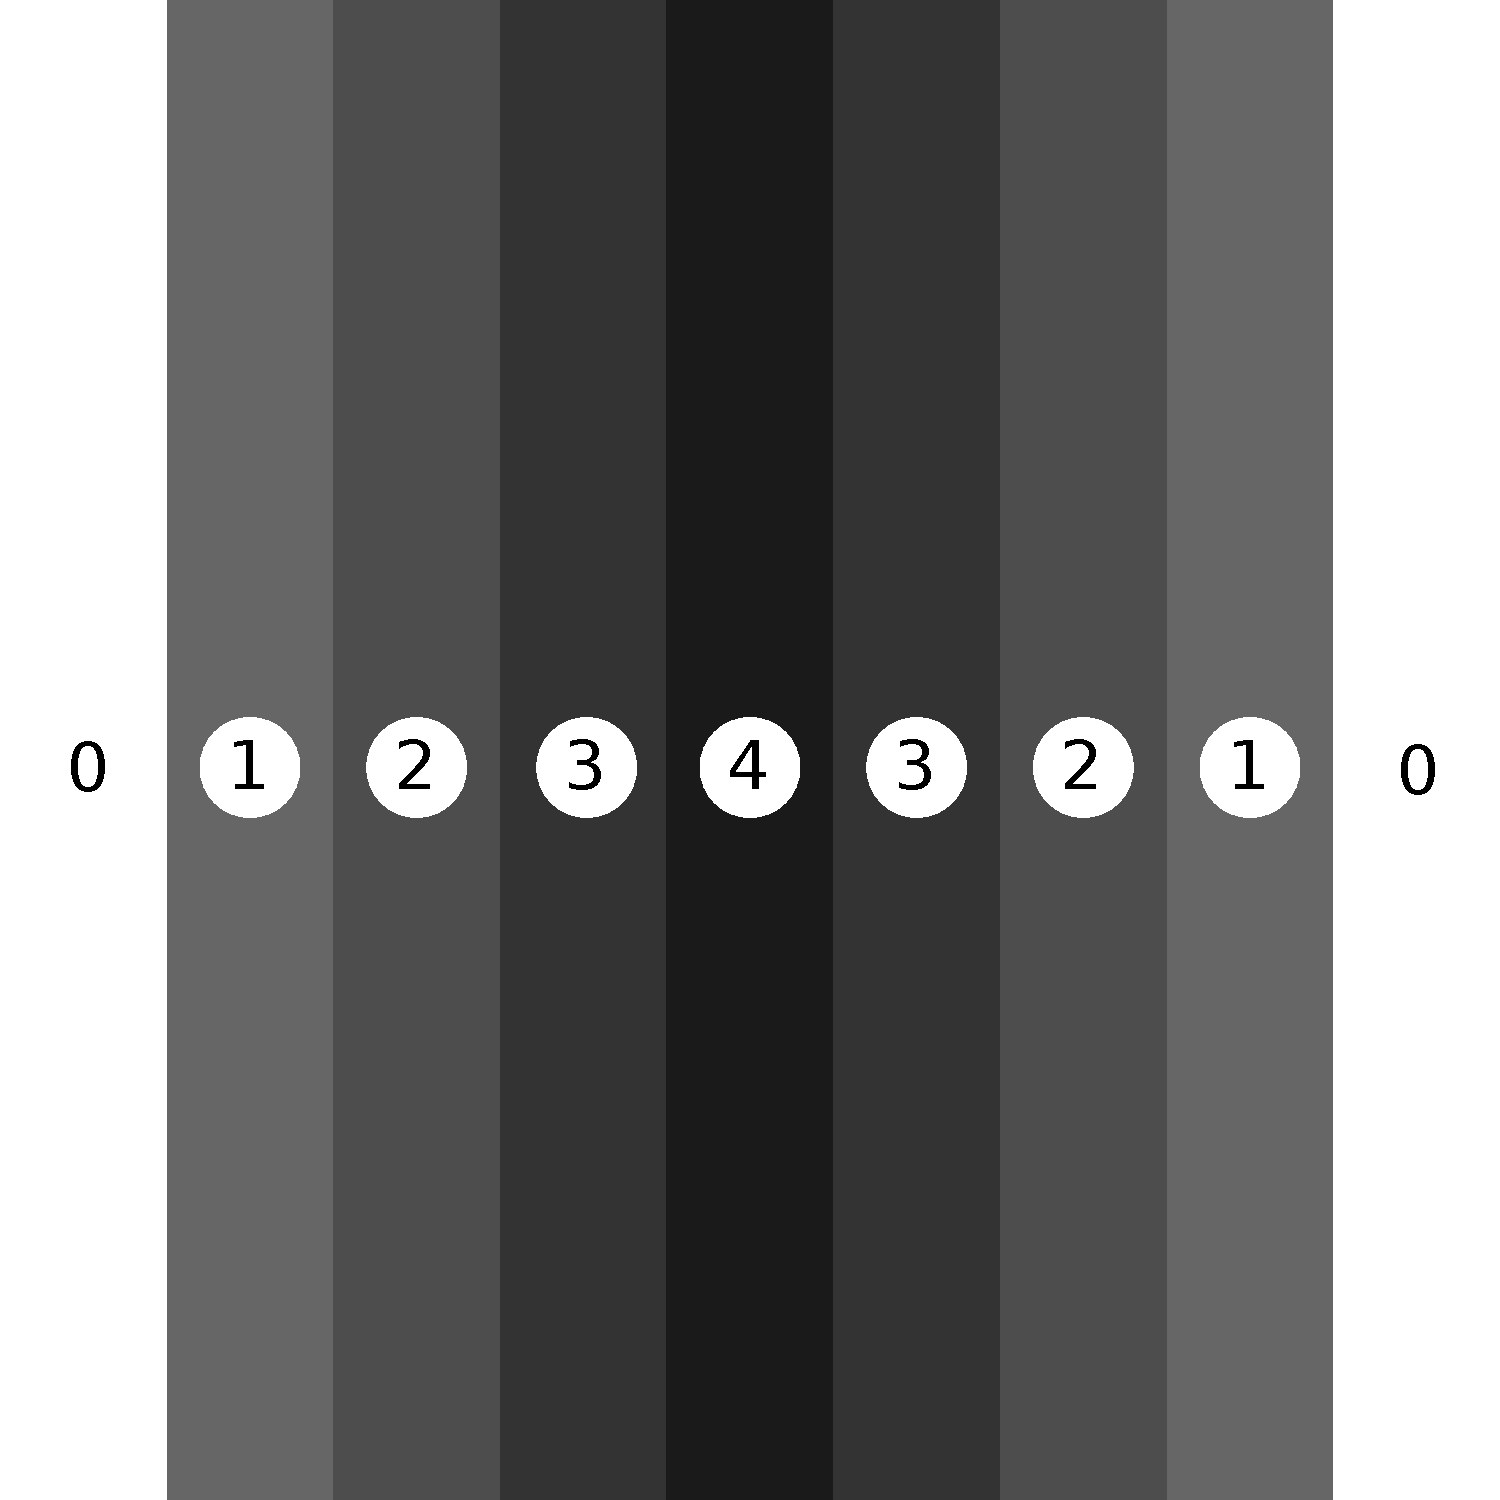
\includegraphics[width=0.2\textheight]{linewidth/line_width}
      \caption{A representation of a line that is seven pixels wide, broken down into reach region with different zero-distances}
      \label{lineseven}
    \end{subfigure}

    \begin{subfigure}[B]{0.9\textwidth}
      \centering
      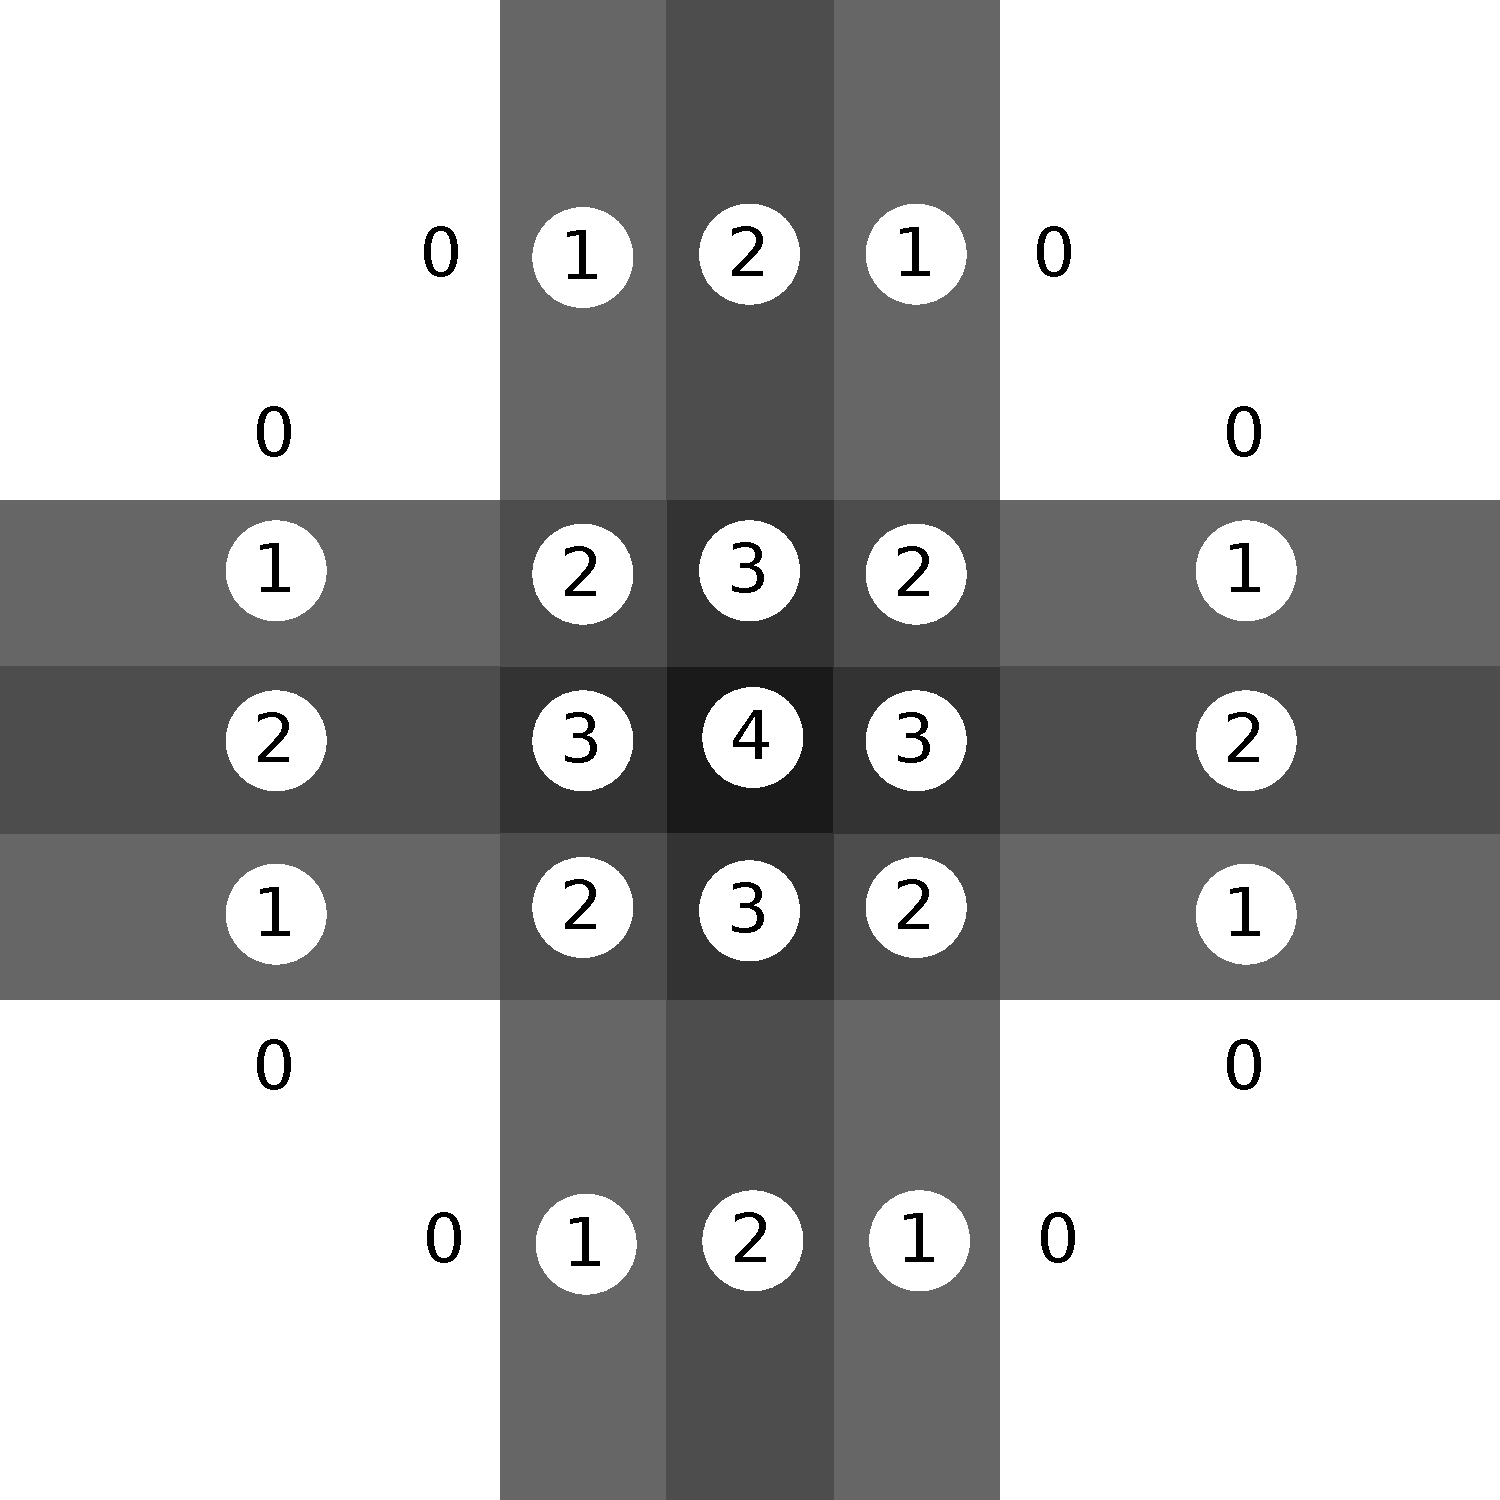
\includegraphics[width=0.2\textheight]{linewidth/line_width_cross}
      \caption{Two intersecting lines, that are 3 pixels wide. The point of intersection produces a maximum zero-distance of 4}
      \label{linecross}
    \end{subfigure}
    \caption{Two examples of lines with their zero-distances calculated.}
    \label{linewidthexamples}
  \end{figure}

  A more complicated method, described below, relies on two statistical properties of the image;
     the average distance of the pixels, and standard deviation of each pixel from the average distance.
  \subsection{Average Distance to a Zero Valued Pixel}
    By simple inspection of figure \ref{lineseven}, it is clear that the average distance is dependent upon something approaching a sum of incremental integers.
    Lines with even and odd widths will differ slightly; even values have two maximum zero-distances, odd values only have one.
    This can be seen in equation \ref{pixeldistanceexample}, where PixelDistance$(n)$ lists the zero-distances in an $n$ pixel wide line.
    \begin{align}
      \text{PixelDistances}(4) &= \{1,2,2,1\}\notag\\
      \text{PixelDistances}(5) &= \{1,2,3,2,1\}\notag\\
      \text{PixelDistances}(6) &= \{1,2,3,3,2,1\}
      \label{pixeldistanceexample}
    \end{align}
    For a general $N$-pixel wide line, the sum of all values is in the range $[0,N/2]$ on one side, and $[N/2,0]$ on the other.
    This has the mathematical form of a geometric series.
    This geometric can be conveniently expressed as simple formula, described in equation \ref{geometricsum}.
    \begin{equation}
      \text{Sum}(N):=\sum_{i=0}^{N} i = \frac{N(N+1)}{2}
      \label{geometricsum}
    \end{equation}
  
    First, we consider even valued widths, as this is the simplest case.
    This is can be calculated as twice the sum of integers in the range $[0,N/2]$, as seen in equation \ref{sumeven}.
    \begin{align}
      \text{EvenSum}(N):&=2\text{ Sum}(N/2)\notag\\
                        &=2\sum_{i=0}^{N/2}i\notag\\
                        &=2\frac{(N/2)(N/2+1)}{2}\notag\\
                        &=N\left(\frac{N}{4}+\frac{1}{2}\right)\notag\\
                        &=\frac{N^2+2N}{4}\
      \label{sumeven}
    \end{align}
    For an odd-valued $N$, the sum is in the range $[0,(N+1)/2]$ and $[(N-1)/2,0]$.
    This can be reduced to twice the sum of integers in the range $[0,(N-1)/2]$ plus $(N+1)/2$, shown in equation \ref{sumodd}.
    \begin{align}
      \text{OddSum}(N):&=\frac{N+1}{2}+2\text{ Sum}((N-1)/2)\notag\\
                        &=\frac{N+1}{2}+2\sum_{i=0}^{(N-1)/2}i\notag\\
                        &=\frac{N+1}{2}+2\frac{((N-1)/2)((N-1)/2+1)}{2}\notag\\
                        &=\frac{N+1}{2}+\frac{N-1}{2}\frac{N+1}{2}\notag\\
                        &=\frac{N+1}{2}\frac{N+1}{2}\notag\\
                        &=\frac{N^2+2N+1}{4}
      \label{sumodd}
    \end{align}

    These values are very close, differing by only $\frac{1}{4}$ of a pixel.
    When these formulas are used to calculate the average zero-distance, this difference further decreases.
    Equation \ref{avgdistwidth} demonstrates this.
    The estimation formula loses reliability for $N<1$. 
    As pixels are positioned on a discrete grid, the only possible value for $N<1$ is zero, which represents no line.

    \begin{align}
     \text{AvgDist}(N) :&=
        \begin{cases}
          \frac{\text{EvenSum}(N)}{N} =\frac{1}{4}\left(N+2\right) \text{ if } N \text{ even}\\
          \frac{\text{OddSum}(N)}{N} =\frac{1}{4}\left(N+2+\frac{1}{4N}\right) \text{ if } N \text{ odd}
        \end{cases}\notag\\
      &= \frac{N+2}{4} + \text{O}(N^{-1})
      \label{avgdistwidth}
    \end{align}

    For large values of $N$, the average distance approaches the EvenSum formula.
    This can be seen in figure \ref{oddevenwidth}.
    The background shading represents the values bounded by the values of OddSum and EvenSum.
    The figure also shows that the maximum error for any given value of $N$ is at most a quarter of a pixel.

    \begin{figure}[H]
      \centering
      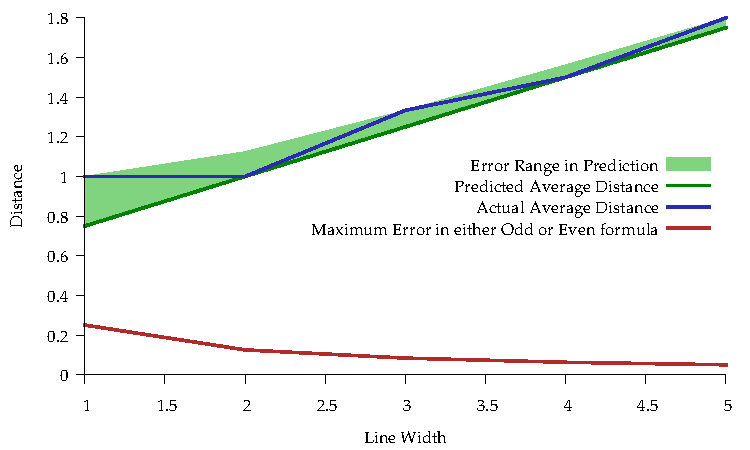
\includegraphics[width=0.9\textwidth]{graphs/oddevenwidth.pdf}
      \caption{Graph showing the estimation of the average distance to a zero valued pixel using the Odd and Even formulae.}
      \label{oddevenwidth}
    \end{figure}

    Equation \ref{avgdistwidth} shows that there is an approximately linear relationship between the average zero-distance and the width of the line drawn.
    It is possible to invert this equation.
    This produces a formula, equation \ref{linewidtheq}, to calculate line width from the average zero-distance.

    \begin{equation}
      \text{LineWidth}(avg) := \text{AvgDist}^{-1}(avg) = \frac{avg-0.5}{0.25}
      \label{linewidtheq}
    \end{equation}

    Using this equation, the line width can be approximated using an easily calculable property of the image; the average distance to a zero-valued pixel.
    The maximum error in equation \ref{avgdistwidth} was a quarter of a pixel.
    Equation \ref{linewidtheq} accordingly has an maximum error of 1 pixel (at $N=1$).
    The formula has a minimum error of 0 for all even valued widths.
    An unusual effect of this is that the method cannot determine a difference between a line of width 1 pixel and a line of width 2.
    This means that this method can be used only as a upper bound on the scaling between two images.

  \subsection{Standard Deviation in Distance to Zero Valued Pixels}
    The line width can also be deduced from another calculable property of the system; the standard deviation.
    Standard deviation, here, is defined to be the normalised deviance of all pixels from the average position of each pixel, $x_i$.
    \[\text{StdDev}(N) := \sqrt{\frac{\sum \left(x_i-\text{AvgDist}(N)\right)^2}{N}}\]
    
    To simplify the mathematics, we act on summation for now.
    We will call this operand Deviance.
    \[\text{Deviance}(N) := \sum_{i=0}^N\left(x_i-\text{AvgDist}(N)\right)^2 =
      \begin{cases}
        DevEven(N) \text{ if } N \text{ is even}\\
        DevOdd(N) \text{ if } N \text{ is odd}
      \end{cases}
    \]
    As before, $x_i$ will take values from $[0,..,N,...0]$, and AvgDist$(N)$ is defined in equation \ref{avgdistwidth}.
    We will show the method for finding the standard deviation for even valued widths, odd values follow from above.
    We can now write this equation (ignoring the nominal differences between odd and even values of $N$) as
    \begin{align}
      \text{DevEven}(N) &= 2\sum_{i=0}^{N/2}\left(i-\frac{N+2}{4}\right)\notag\\
        &=2\sum_{i=0}^{N/2}\left(i^2-2i\frac{N+2}{4}+\frac{(N+2)(N+2)}{16}\right)\notag\\
        &=2\left(\sum_{i=0}^{N/2}(i^2)-2\frac{N+2}{4}\sum_{i=0}^{N/2}(i) + \sum_{i=0}^{N/2}\left(\frac{(N+2)(N+2)}{16}\right)\right)\notag\\
        &=2\left(\sum_{i=0}^{N/2}(i^2)-\frac{N+2}{4}\frac{N(N/2+1)}{2} + \frac{N}{2}\frac{(N+2)(N+2)}{16}\right)
      \label{devianceunfin}
    \end{align}
    
    The sum in equation \ref{devianceunfin} is, as with equation \ref{geometricsum}, easily expanded using geometric identities.
    In this case, the formula is described in equation \ref{geometricsumsq}.
    \begin{equation}
      \sum_{i=0}^N i^2 = \frac{1}{6}N(N+1)(2N+1)
      \label{geometricsumsq}
    \end{equation}
    We can now continue expanding DevEven$(N)$;
    \begin{align}
      \text{DevEven}(N) &= \frac{1}{3}\frac{N}{2}(N/2+1)(N+1) - \frac{N(N+2)(N+2)}{4}+\frac{N(N+2)(N+2)}{16}\notag\\
        &=...\notag\\
     ...&=\frac{1}{48}\left(N^3-4N\right)
    \end{align}
    Using this formula for DevEven, we can now calculate the standard deviance.
    \begin{align}
      \text{StdDevEven}&=\sqrt{\frac{\text{DevEven}(N)}{N}}\notag\\
        &=\sqrt{\frac{N^3-4N}{48N}}\notag\\
        &=\frac{N}{4\sqrt{3}}+O(\sqrt{N})
      \label{evenstddev}
    \end{align}
    Using similar calculations for odd widths, StdDevOdd has a value of
    \begin{align}
      \text{StdDevOdd}&=\sqrt{\frac{\text{DevOdd(N)}}{N}}\notag\\
        &=\sqrt{\frac{N^2}{16N}+\frac{N^2-3N+2}{48N}}\notag\\
        &=\frac{N}{4\sqrt{3}}+O(\sqrt{N})
      \label{oddstddev}
    \end{align}
  
    As these functions are equivalent (up to O$(\sqrt{N})$), we define the Standard Deviation approximation as
    \begin{equation}
      \text{StdDev}(N):=\frac{N}{4\sqrt{3}}
      \label{stddevapprox}
    \end{equation}

    Figure \ref{stddevwidth} shows the comparison of these formulae with actual data.
    The data and approximate standard deviation are well bounded inside the Odd and Even standard deviations.
    The maximum error that can be expected from the approximation is less than 0.3 pixels.
    This is at the boundary case of 2 width pixels.
    At all other points, the error is a small fraction of the actual value.

    \begin{figure}[H]
      \centering
      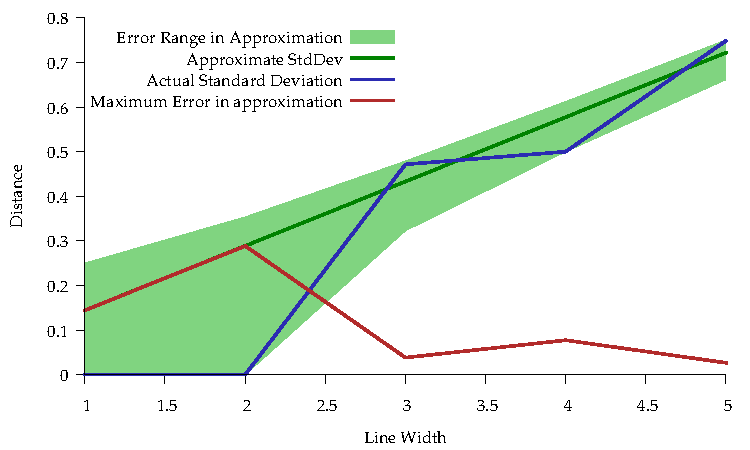
\includegraphics[width=0.9\textwidth]{graphs/stddevwidth.pdf}
      \caption{Graph showing the relationship between line width and the Standard Deviation of pixel distance to zero valued pixels.}
      \label{stddevwidth}
    \end{figure}

    Again, as a linear formula has been produced, the relationship can be reversed, to get line width from standard deviation.
    \begin{equation}
      \text{LineWidth}(stddev) := \text{StdDev}^{-1}(stddev) = 4\sqrt{3}\cdot stddev
      \label{linewidthstddev}
    \end{equation}
    Equation \ref{linewidthstddev} can not give an exact estimation of line widths; it will overestimate odd widths and underestimate even widths.
    For the correct standard deviation, it will give the correct line width to within $\pm1$ pixel, for all values.
    Thus the standard deviation method can put an upper bound on the scaling between two images.

  \subsection{Combining the Methods}
    Each of these methods is flawed when introduced into an image with overlapping lines, as in figure \ref{linecross}.
    This can be compensated for by successively removing the pixels with the largest distance from the map. %% too long
    At some point during this removal, it is expected that a "sane" mask will be produced.
    A sane mask, in this case, is a mask that displays only the boundary lines of an image.
    For example, a filled in square would be reduced to the 4 border lines that define it's shape.
    A visual example can be seen in figure \ref{sanemasking}.
    The sane mask should produce the most correct line width estimations from either formula.
    Determining which mask is the sane one is not immediately obvious, but can be deduced using a combination of both methods.

    \begin{figure}[H]
      \centering
      \begin{subfigure}[B]{0.9\textwidth}
        \centering
        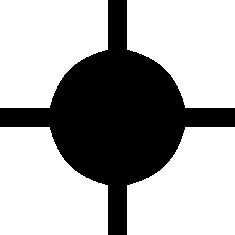
\includegraphics{original_mask}
        \caption{The original image, with an equation distorting solid block of black in the center}
      \end{subfigure}

      \begin{subfigure}[B]{0.9\textwidth}
        \centering
        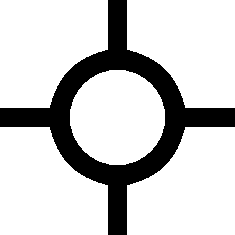
\includegraphics{sane_mask}
        \caption{The sane mask, replacing solid circle in the center with it's border}
      \end{subfigure}

      \begin{subfigure}[B]{0.9\textwidth}
        \centering
        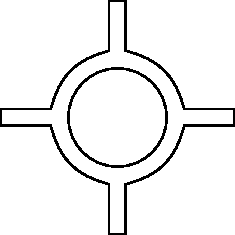
\includegraphics{unsane_mask}
        \caption{The image after too many maxima have been removed, which would also distort the equation}
      \end{subfigure}
      \caption{A representation of the removal of the highest zero-distance pixels, to reveal a sane mask}
      \label{sanemasking}
    \end{figure}

    Each method reacts differently to the removal of the largest zero-distance pixels.
    This can be seen in figure \ref{stddev_image}, the mean and the standard deviation have very different responses.
    These differences allow a combination of the two methods; only when they agree can a mask be described as sane. 
      \begin{figure}[H]
        \centering
        \begin{subfigure}[B]{0.8\textwidth}
          \centering
          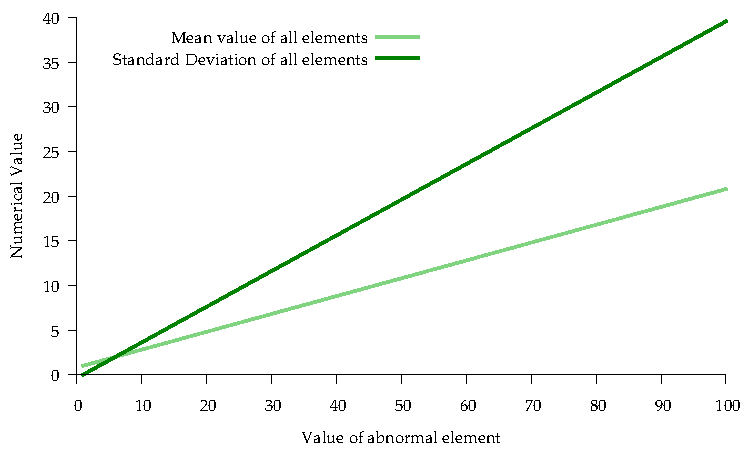
\includegraphics[width=0.9\textwidth]{graphs/stddev_great_abnormal}
          \caption{Changing the value of a single abnormal element in a list}
        \end{subfigure}

        \begin{subfigure}[B]{0.8\textwidth}
          \centering
          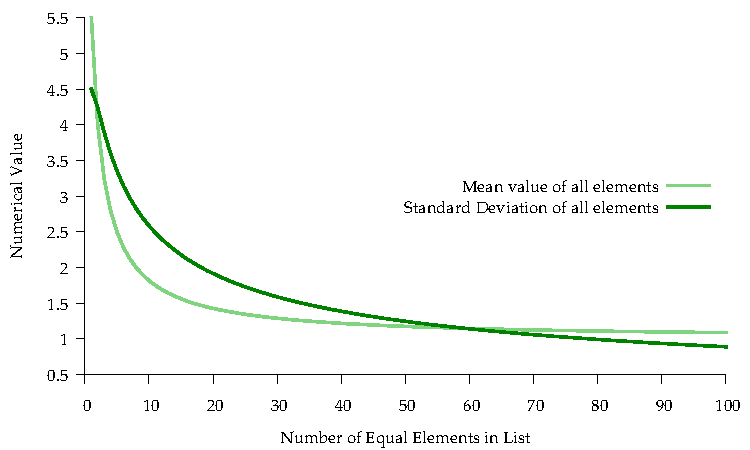
\includegraphics[width=0.9\textwidth]{graphs/stddev_great_range}
          \caption{Changing the ratio of normal data to abnormal data}
        \end{subfigure}
        \caption{The response of mean and standard deviation to various types of erroneous data}
        \label{stddev_image}
      \end{figure}
    
    It is unlikely a perfectly sane mask will be located.
    In this case, the mask with the minimal difference between the two estimations of line width will be the sane mask.
    The average of the two methods will be the line width estimation used.
    The line width is reliable to the nearest integer, rounded up, except in the case that the line width is 1 pixel.
    This is because a 1 pixel width line is indistinguishable from a 2 pixel width line, using the mean and standard deviation.
    To demonstrate this, we define $Z_n$ as the list of zero distances of each pixel in the slice of an $n$ wide pixel.
    \[ Z_1 = \{1\},\,Mean(Z_1) = 1,\, StdDev(Z_1) = 0\]
    \[ Z_2 = \{1,1\},\,Mean(Z_2) = 1,\, StdDev(Z_2) = 0\]
    This being the case, a 1 pixel line may be interpreted to be a 3 pixel line.
    Using this method, a maximum line width can be estimated.
    Comparing these line widths, the scaling between two cartoon images can be approximated.
    \subsection{Testing}
      This method was tested with an image with several thickness.
      The base image contains vertical lines that are increasingly further apart from each other, with lines connecting each point.
      This can be seen in figure \ref{solid_linewidth}.
      There are two types of test, solid lines, which have clearly defined boundaries, and aliased lines, which are more realistic.
      The results of using this method of each of these images is listed in table \ref{linewidthtable}
      The line widths are almost all correctly predicted to within 1 pixel, with the exception of 1 pixel on a solid line.
      As discussed earlier, this has been anticipated.
    \begin{figure}[H]
      \centering
      \begin{subfigure}[B]{0.19\textwidth}
        \centering
        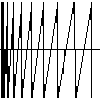
\includegraphics[height=0.1\textheight]{linewidth/linewidth_1_solid.png}
        \caption{1 pixel solid}
      \end{subfigure}
      \begin{subfigure}[B]{0.19\textwidth}
        \centering
        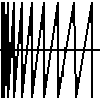
\includegraphics[height=0.1\textheight]{linewidth/linewidth_2_solid.png}
        \caption{2 pixel solid}
      \end{subfigure}
       \begin{subfigure}[B]{0.19\textwidth}
        \centering
        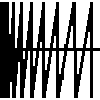
\includegraphics[height=0.1\textheight]{linewidth/linewidth_3_solid.png}
        \caption{3 pixel solid}
      \end{subfigure}
     \begin{subfigure}[B]{0.19\textwidth}
        \centering
        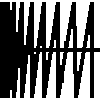
\includegraphics[height=0.1\textheight]{linewidth/linewidth_4_solid.png}
        \caption{4 pixel solid}
      \end{subfigure}

      \begin{subfigure}[B]{0.19\textwidth}
        \centering
        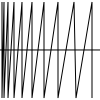
\includegraphics[height=0.1\textheight]{linewidth/linewidth_1_blur.png}
        \caption{1 pixel aliased}
      \end{subfigure}
      \begin{subfigure}[B]{0.19\textwidth}
        \centering
        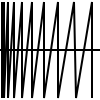
\includegraphics[height=0.1\textheight]{linewidth/linewidth_2_blur.png}
        \caption{2 pixel aliased}
      \end{subfigure}
       \begin{subfigure}[B]{0.19\textwidth}
        \centering
        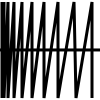
\includegraphics[height=0.1\textheight]{linewidth/linewidth_3_blur.png}
        \caption{3 pixel aliased}
      \end{subfigure}
     \begin{subfigure}[B]{0.19\textwidth}
        \centering
        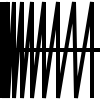
\includegraphics[height=0.1\textheight]{linewidth/linewidth_4_blur.png}
        \caption{4 pixel aliased}
      \end{subfigure}
      \caption{
        Images used to test \texttt{estimate\_black\_line\_thickness}.
        They are designed to stress estimation, with lines that overlap regularly.
        The top row are solid pixels, with clear boundaries.
        The bottom row show aliased lines, which are more realistic.
      }
      \label{solid_linewidth}

    \end{figure}
    \begin{figure}[H]
      \centering
      \begin{tabular}{|c|c|c|}
        \hline
        Line Width&Solid Line Predicted Width&Aliased Line Predicted Width\\
        \hline
        1&2.42688&1.31487\\
        \hline
        2&2.74886&2.75531\\
        \hline
        3&3.05320&2.87646\\
        \hline
        4&4.21705&4.33824\\
        \hline
      \end{tabular}
      \caption{
        A comparison of the line width analysis technique on images from \ref{solid_linewidth}
        All but one of the values are within 1 pixel of the actual value.
        The anomalous 1 pixel result can be mistaken as a 2 pixel width.
        The technique cannot guarantee distinction between 1 and 2 pixels.
      }
      \label{linewidthtable}
  \end{figure}

  \subsection{Parallelism}
    Analysing the line width is a parallelisable task.
    Calculating the zero-distance of each pixel in the map needs to be done in serial.
    This is because bisecting a line could make a large change to the standard deviation, if there aren't many lines.
    The bisection can't easily be avoided without knowing the width of the lines, so using halo data is not viable.
    However, splitting the mask after the zero-distance has been calculated is parallelisable.
    The average can be calculated with a reduction operation, as can the summation of the standard deviation.
    The overhead of using OpenMP for small images is likely to reduce usefulness of parallelism.
    Large images may benefit from this.

    \begin{figure}[h]
      \centering
      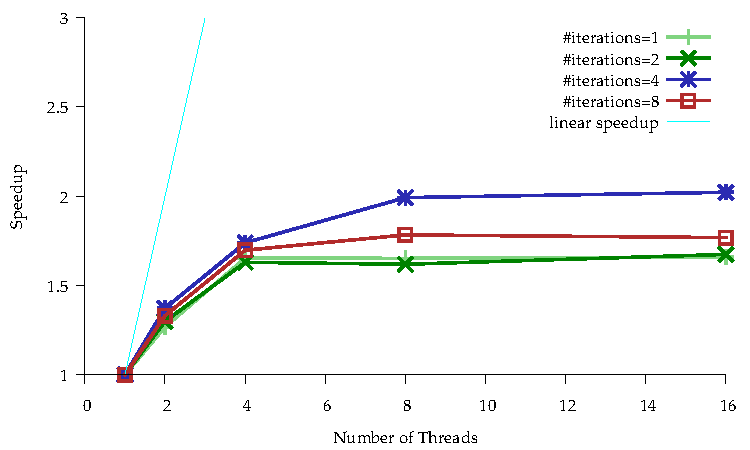
\includegraphics{benchmark/thickness_benchmark.pdf}

      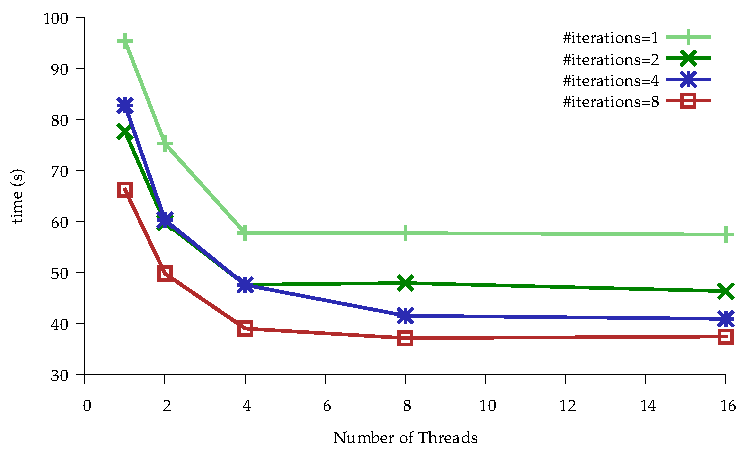
\includegraphics{benchmark/thickness_time.pdf}
      \caption{Speedup of line width analysis due to parallelism}
      \label{thicknessbenchmark}
    \end{figure}
    \textit{I will put in some results here when I put them together}
    \biblio

\end{document}
